% Use only LaTeX2e, calling the article.cls class and 12-point type.

\documentclass[12pt, notitlepage, letterpaper]{article}
\usepackage{bm,url,graphicx, amsfonts, amssymb} %PJM added these here
\usepackage{amsmath}    % need for subequations
\usepackage{graphicx}   % need for figures
\usepackage{subfigure}  % use for side-by-side figures


% The following parameters seem to provide a reasonable page setup.

% Include your paper's title here

\title{MA731: HW5}

\author{Thomas Richardson}
{\large }

% Include the date command, but leave its argument blank.

% \date{\small}



%%%%%%%%%%%%%%%%% END OF PREAMBLE %%%%%%%%%%%%%%%%



\begin{document}

% Double-space the manuscript.

\baselineskip 24pt

% Make the title.

\maketitle

\noindent

\paragraph{Parts i, ii:}

Our system is as follows:

%Equations for original system
\begin{equation}
\label{eq:sys01}
\dot{x} = 0.5x + 3u
\end{equation}

\begin{equation}
\label{eq:cost}
J(x(t)) = \frac{1}{2}\int_{0}^{10}[x^2 + 6u^2] dt  + 5x(10)^2
\end{equation}

\noindent For the first two sections, the optimal control corresponding to the above system, $u^*$, was found and then used to simulate the progression of the system by using it as an input to Eq \ref{eq:sys01}.  An expression for obtaining $u^*$ at various points in time was obtained by deriving the necessary conditions from the Hamiltonian constructed from Eqns \ref{eq:sys01} and \ref{eq:cost}, and then solving the BVP associated with the system and the given initial condition (see Eq \ref{eq:BVP01}).  Using the derived expression,  Eq \ref{eq:sys01} was solved with a numerical integrator and $u^*$ as an input.  The the results from the BVP used to obtain $u^*$ are in Fig \ref{fig:BVP}, and the simulated trajectory utilizing $u^*$ is shown in Fig. \ref{fig:OrigSys}.  We see that the final values of the trajectories differ slightly in the two plots, indicating that the results obtained from the two systems should not be expected to be the same in practice.

%Equation for BVP input in MATLAB
\begin{align}
\label{eq:BVP01}
\begin{pmatrix}
\dot{x} \\
\dot{\lambda}
\end{pmatrix}
&=
\begin{bmatrix}
0.5x - \frac{3}{2}\lambda \\
-x + 0.5\lambda
\end{bmatrix}
&
\hfill \text{BVC}
&=
\begin{bmatrix}
x(0) - 4 \\
10x(10) - \lambda(10)
\end{bmatrix}
\end{align}

%BVP figure for the original system, control
\begin{figure}[h]
\begin{center}
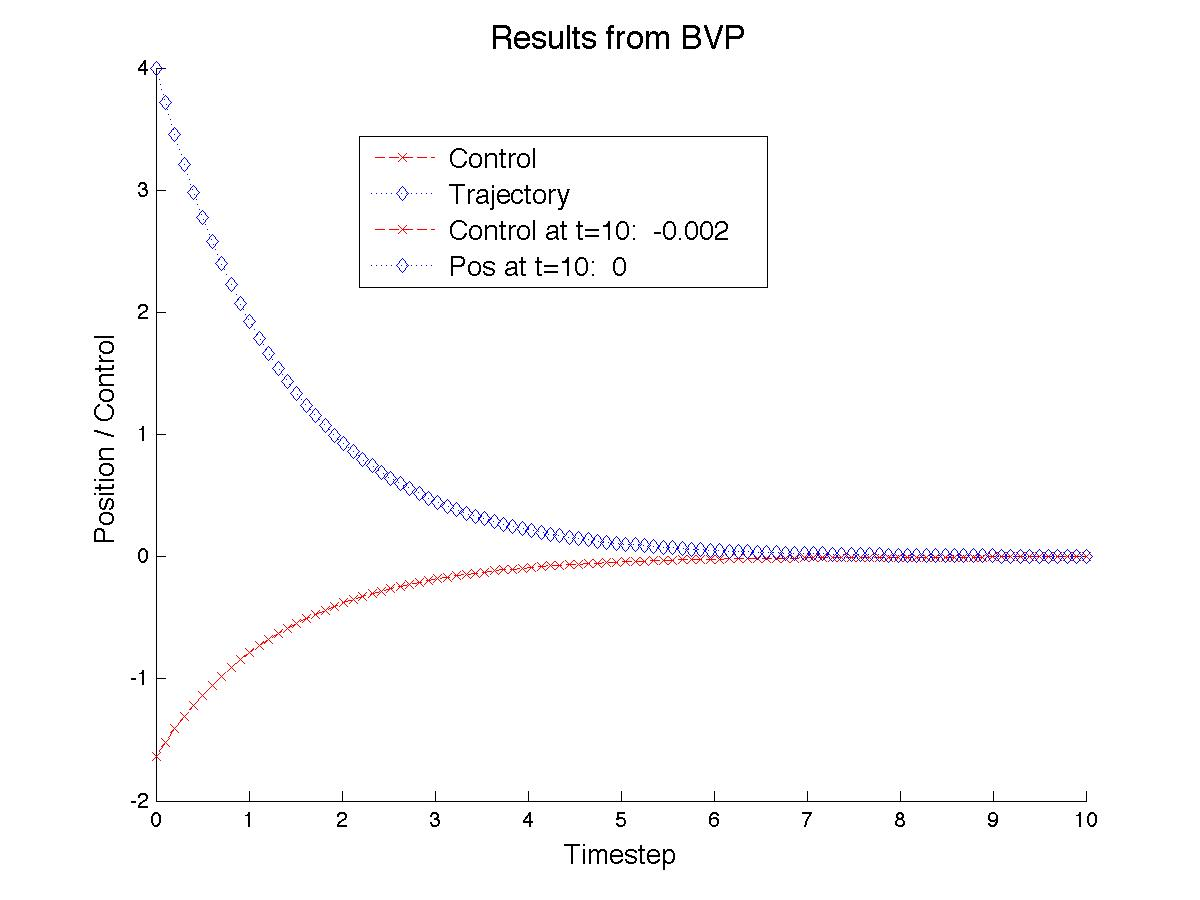
\includegraphics[width=4in]{BVPOrig}
\caption{\label{fig:BVP} Results from the BVP system, Eq \ref{eq:BVP01}}
\end{center}
\end{figure}

%First figure for the original system, control
\begin{figure}[h]
\begin{center}
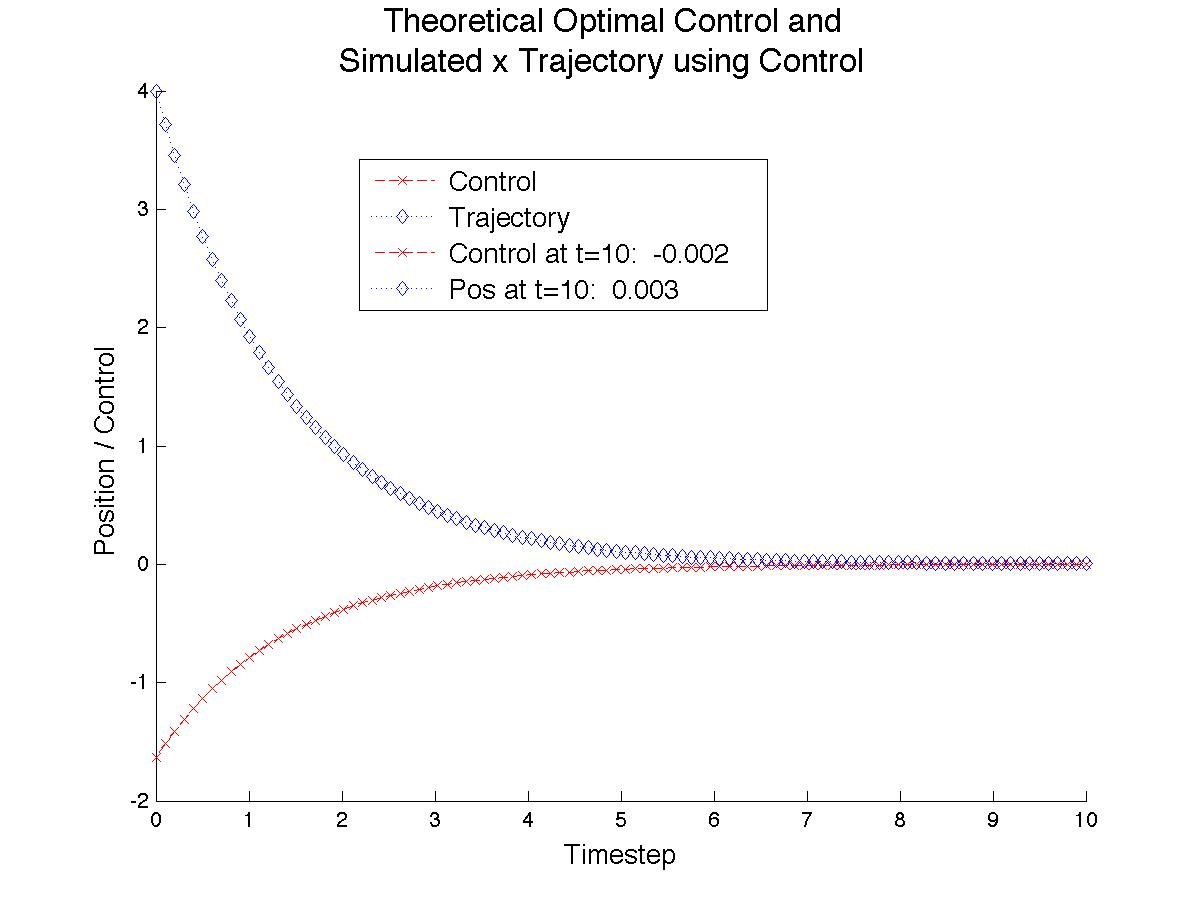
\includegraphics[width=4in]{OpenTrajCont0to10}
\caption{\label{fig:OrigSys} Plot of $u^*$ and Trajectory from Eq \ref{eq:sys01} with $u^*$ as input}
\end{center}
\end{figure}

\paragraph{Parts iii, iv:}

For these portions, we used the same system described by Eqns \ref{eq:sys01} and \ref{eq:cost}, but instead developed a feedback control by calculating the Kalman Gain for the system, instead of using an open loop control.  To do this, we first needed to calculate an expression for $S$ (see Eqns \ref{eq:Kalm} and \ref{eq:S}) that we could evaluate at various points in time on the $[0,10]$ interval.  With this $S$, we could then simulate Eq \ref{eq:sys01}, replacing $u^*$ with the control obtained from the Kalman Gain to obtain Eq \ref{eq:sys02}.  In order to calculate $S$ along the trajectory, we needed to first solve Eq \ref{eq:S}.  We solved this as a BVP since we know the parameter's final value, $S(10) = 10$, from the boundary conditions in Eq \ref{eq:BVP01}.  After solving this system and then simulating the trajectory for Eq \ref{eq:sys02} using the obtained expression, we obtain Fig \ref{fig:KalmSys}.  It turns out that the solution obtained from the Kalman Gain is not optimal with regards to the cost function.  The cost of the simulation using $u^*$ is about 25 units, while the cost of the simulation using the Kalman Gain is about 26 units.  In the following sections, we see the benefits of using Kalman Gain.

\begin{equation}
\label{eq:Kalm}
K = R^{-1}B^TS = \frac{1}{2}S
\end{equation}

\begin{equation}
\label{eq:S}
-\dot{S} = A^TS + SA + Q  -SBR^{-1}B^TS= -\frac{3}{2}S^2 + S + 1
\end{equation}

\begin{equation}
\label{eq:sys02}
\dot{x} = (A - BK)x = (\frac{1}{2} - \frac{3}{2}S)x
\end{equation}

%Second figure for the closed system, control
\begin{figure}[h]
\begin{center}
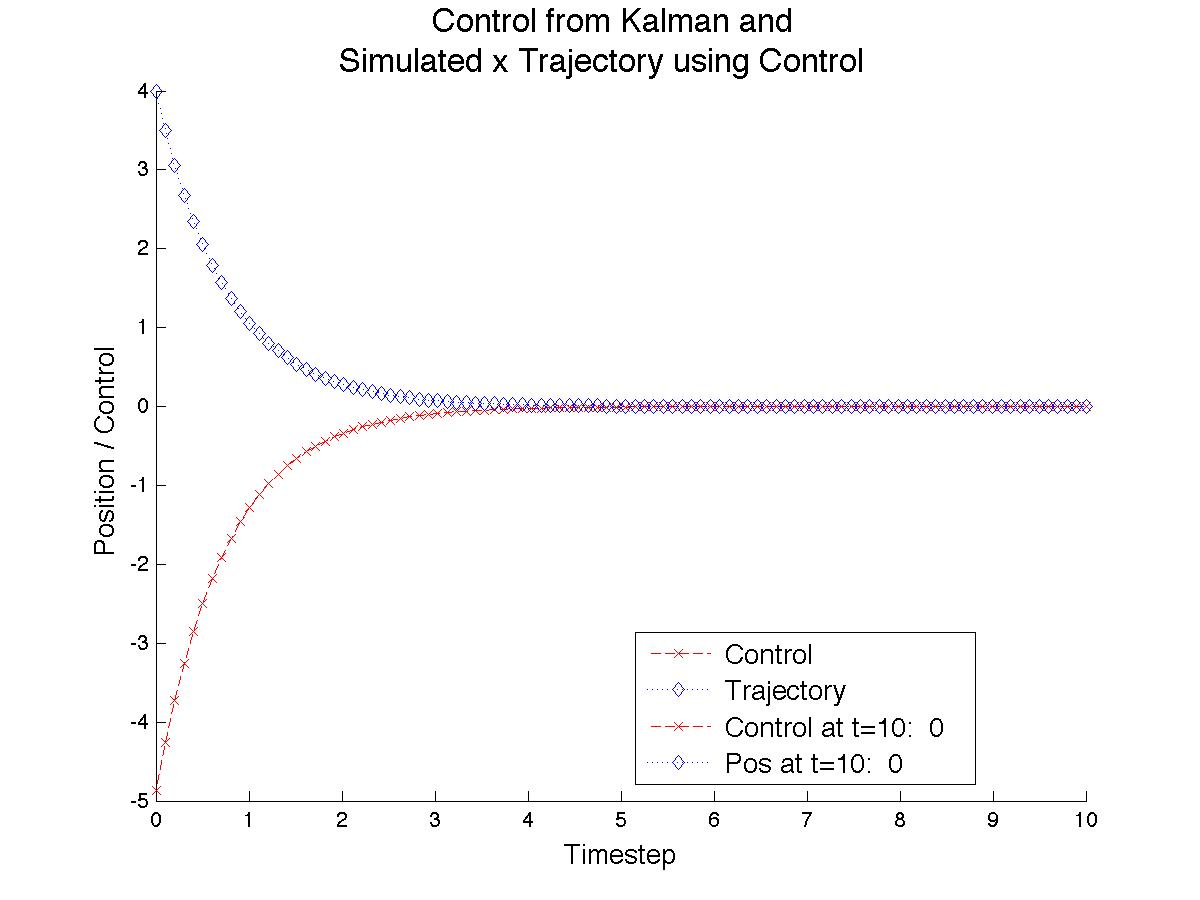
\includegraphics[width=4in]{ClosedTrajCont0to10}
\caption{\label{fig:KalmSys} Plot of $u$ from Kalman Gain and Trajectory from Eq \ref{eq:sys02} }
\end{center}
\end{figure}


\paragraph{Parts v, vi:}

For the last two parts, we use the equations derived in the previous parts with an additional input, that of an impulse function described by Eq \ref{eq:delta}.  The two systems described in Eqns \ref{eq:sys03} and \ref{eq:sys04} were then simulated on the time span $[0,10]$ to obtain Figs \ref{fig:deltaopen} and \ref{fig:deltaclosed}.  Comparing these two plots, we can clearly observe the benefit granted from the control feedback derived via the Kalman Gain; the system remains well-behaved despite the external disturbance.  These two very different results are to be expected, though, since $u^*$ for the original system is static and designed for a specific course.  When the position is shifted away from this optimal course, $u^*$ is no longer optimal.  Instead, the system has a new static optimal trajectory corresponding to this position.  If we instead run the BVP corresponding to Eq \ref{eq:sys03}, we see that the control calculated is adjusted to cope with the delta function (Fig \ref{fig:OpenBVPDel}).  The obtained control, however, still does stabilize the simulated system, as shown in Fig \ref{fig:BVPDCompare}.  In other words, the open loop method does not provide the means to effectively create a control policy to stabilize the system even if disturbances to the system are known in advance and can be simulated.  This is a very compelling reason for using a closed-loop control in any situation where outside disturbances, known or unknown, are expected and a control policy must be assigned in advance.

\begin{equation}
\label{eq:delta}
\delta = (4)(t>2)(0.5-|t-2.5|)(t<3)
\end{equation}

\begin{align}
\label{eq:sys03}
\dot{x} = 0.5x + 3u + \delta \\ 
\label{eq:sys04}
\dot{x} = (\frac{1}{2} - \frac{3}{2}S)x + \delta
\end{align}

\begin{figure}[h]
\begin{center}
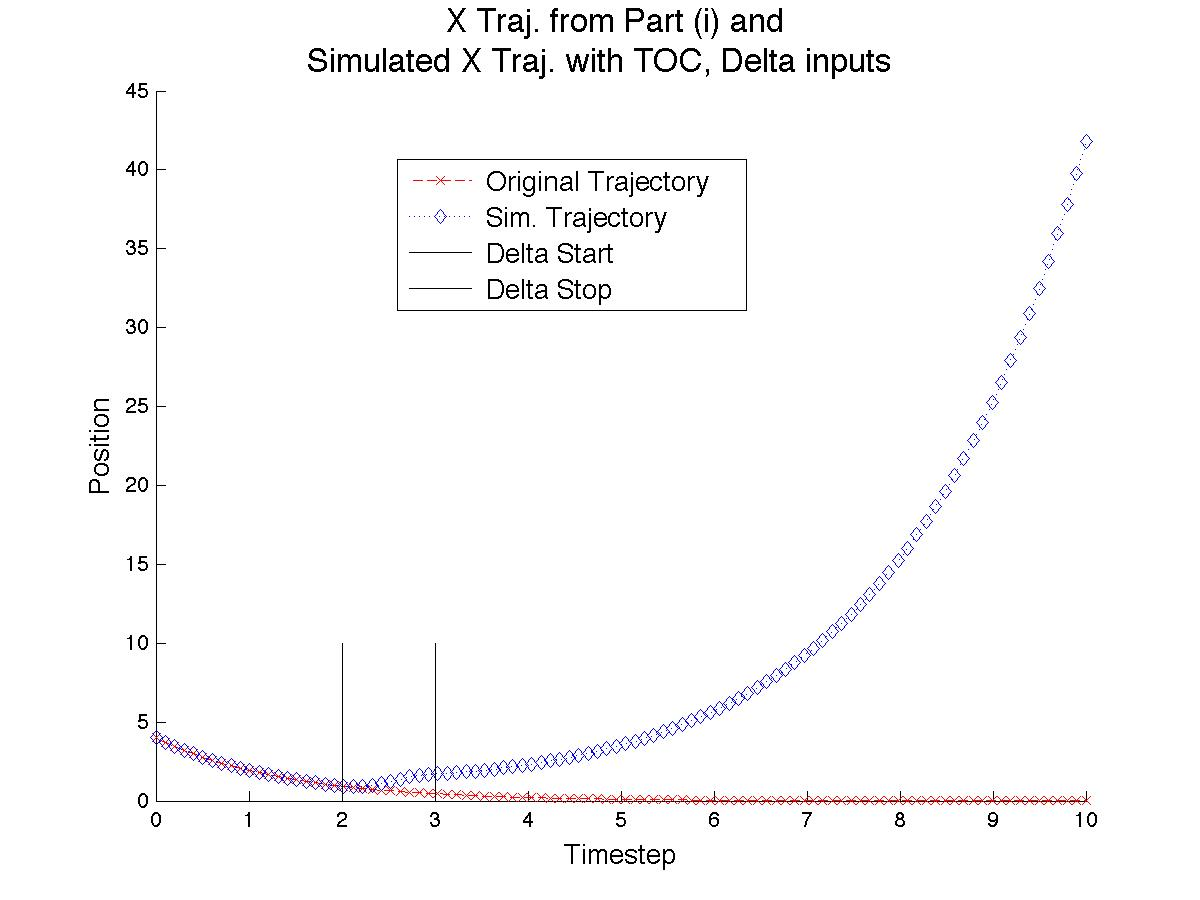
\includegraphics[width=4in]{OpenTrajsDel0to10}
\caption{\label{fig:deltaopen} Orig Sim Traj and Sim. Traj with $u^*$, Delta Input:  Open}
\end{center}
\end{figure}

\begin{figure}[h]
\begin{center}
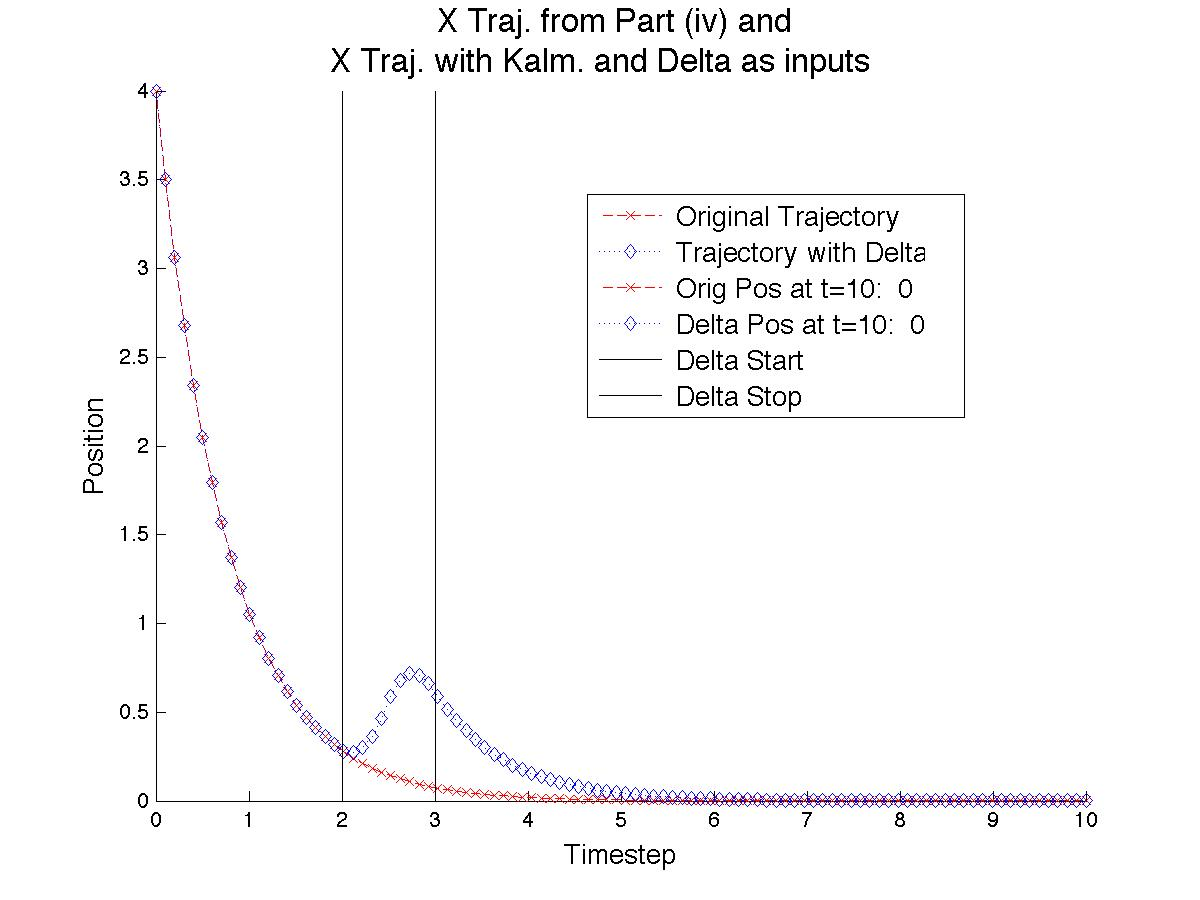
\includegraphics[width=4in]{ClosedTrajsDel0to10}
\caption{\label{fig:deltaclosed} Orig Sim Traj and Sim Traj with Kalm $u$, Delta Input:  Closed}
\end{center}
\end{figure}

\begin{figure}[h]
\begin{center}
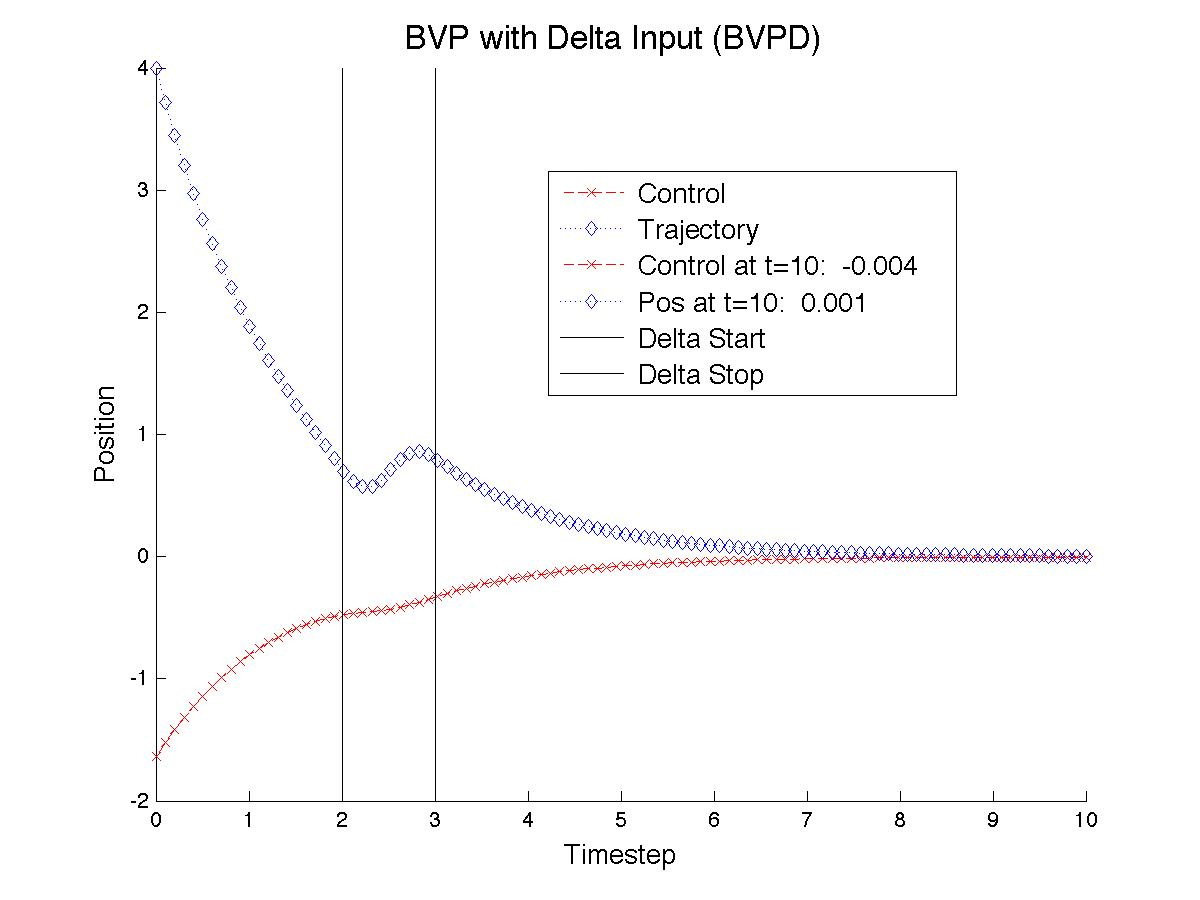
\includegraphics[width=4in]{OpenBVPDel}
\caption{\label{fig:OpenBVPDel} Results from BVP of original system with delta impulse (BVPD)}
\end{center}
\end{figure}

\begin{figure}[h]
\begin{center}
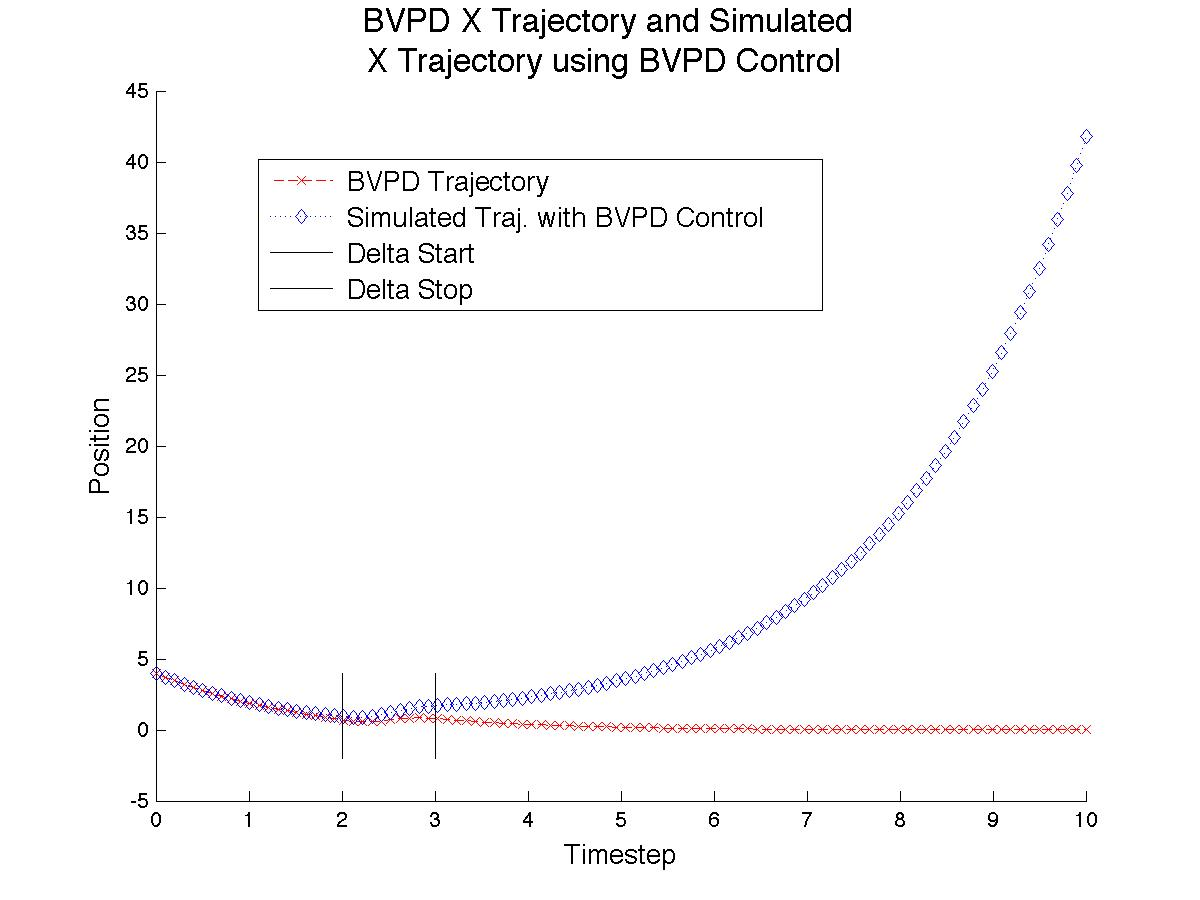
\includegraphics[width=4in]{BVPDCompare}
\caption{\label{fig:BVPDCompare} BVPD Response and Sim Response, BVPD control}
\end{center}
\end{figure}




\end{document}